\chapter{Evaluation}
\label{sec:evaluation}

In this section, we evaluate Sieve's performance
and try to answer one main question: \textit{Is Sieve practical?}

All tests were run on a machine with a 2 GHz
Intel Core i7 and 8 GB of RAM. 
We ran each experiment 50 times, and we report
the average (standard deviations were small).
We configured Sieve to use 2048 bit RSA with
SHA256 for signatures, 128-bit AES in CTR mode
Ed448-Goldilocks elliptic curves in randomized
counter mode for encryption, and ABE using 224-bit MNT curves. 
All web servers ran on the test machine's loopback
network, to minimize network latency and
focus on Sieve's cryptographic overheads.

\begin{figure*}[t!]
\centering
  \subfloat[ABE and Ed448 symmetric key encryption in randomized counter mode.]{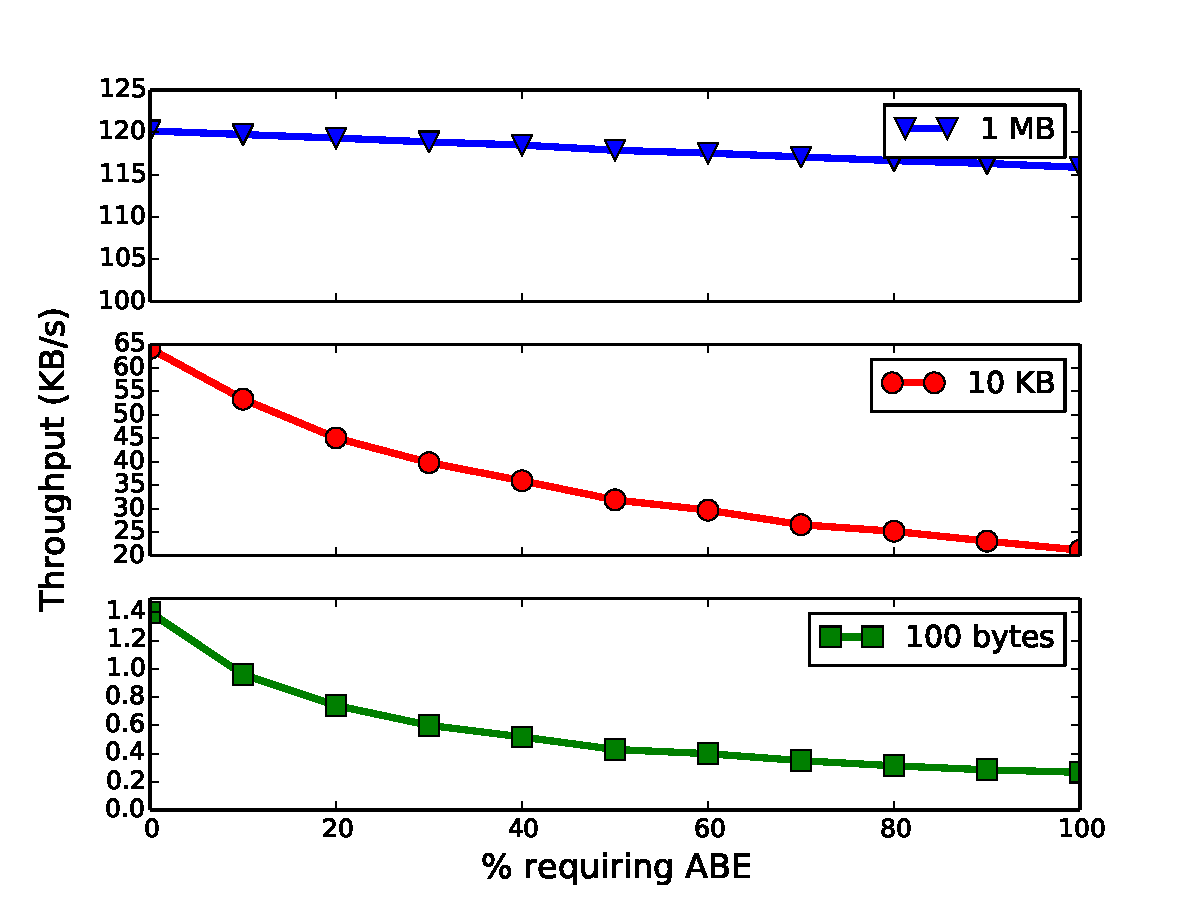
\includegraphics[width=0.48\textwidth]{figs/throughput1.pdf}\label{fig:throughput_ec}}
  \subfloat[ABE and AES symmetric key encryption in CTR mode.]{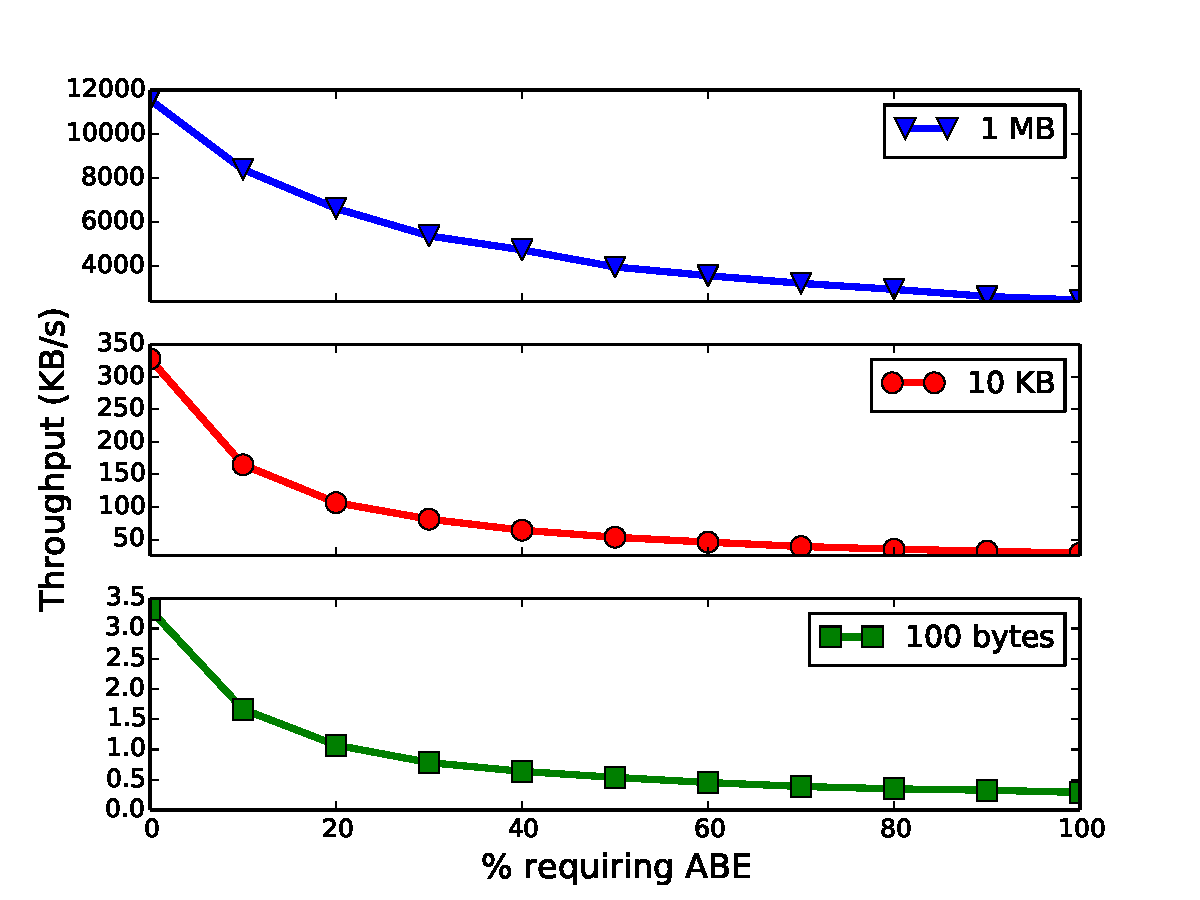
\includegraphics[width=0.48 \textwidth]{figs/throughput2.pdf}\label{fig:throughput_aes}}
    \caption{Throughput of Sieve upload vs. percentage of data blocks
requiring ABE encryption of metadata blocks for a given data upload size. For example,
10 percent requiring ABE operations for 10 KB means that that 1 KB
required the encryption of a metadata
block in addition to symmetric key encryption and 9 KB 
required only symmetric key encryption. We assume there
are 10 attributes for ABE encryption.}
\label{fig:throughput}
\end{figure*}

\section{Uploading and Downloading Data Objects}
When an application uses Sieve, the core
logic of the web service is
unchanged. Thus, the main performance metric
for Sieve is the expense of pushing user data
to the storage provider and pulling user
data into the web service. Ignoring networking
costs, Sieve's overhead is the cryptographic
cost of performing access control checks and
revealing the cleartext data to the third
party.

In Sieve, the user encrypts her data with a symmetric
key $K$, and uses ABE to encrypt the GUID and
$K$. Assuming 64 bit GUIDs, the size of the GUID and AES key
is 24 bytes, and the size of the GUID and Ed448 block cipher key is 64 bytes.~\footnote{
The Ed448 block cipher is 56 bytes compared to AES, which is 16 bytes.
The Ed448 block cipher operates on 56 bytes of cleartext at once
compared to AES, which operates on 16 bytes of cleartext.}  

\subsection{Integrating Sieve with an Existing Health Application:} 
We build Sieve on top of Open mHealth~\cite{omh}, which is an open-source
health application that allows users to analyze and visualize their health data.
We use Open mHealth's data generator to obtain realistic user data in a format
that match current clinical standards. We use Sieve to upload this data to
a storage provider and to download this data into the Open
mHealth health visualizer.

Using Open mHealth, we generate a 
week's worth of fitness and health data, which includes weight,
blood pressure, physical activity, steps taken, and heart rate. 
A day's worth of data has about 14 data points.
The attributes we placed on the data include 
the date, user id, provenance, and type of data.
We imagine a user would 
upload her data daily, and to reduce ABE overhead, the user would create a 
storage-based data structure (\S\ref{sec:minAbeCost}) to store 
a week's worth of a specific type of fitness data, e.g. heart rate. 
The cost to upload a data point on the first day of the week, 
i.e. create a storage-based data structure, is 1.1 s,
using either AES or Ed448 as the symmetric encryption scheme
because ABE represents a majority of the cost. For each subsequent
daily update or update to a pre-existing data point, 
it costs 38.5 ms per data point for Ed448
encryption and 17.1 ms per data point for AES encryption. 

Using Sieve, we download data from the storage provider into the Open mHealth
fitness visualizer. The cost to download the whole data structure (metadata block,
indirect GUIDs table, and data) containing a week's 
worth of data is 0.95 s. To download any updates from the data structure takes 0.25 s
using Ed448 as the symmetric encryption scheme and 0.04 s using AES. 
We note that the user and web service can reduce overall cost by uploading
and downloading data asynchronously or in batches.

\subsection{Microbenchmarks:}
Open mHealth gives us a realistic application for Sieve, but
the size of the data blocks varies depending on the web service.
For example, GPS coordinates for running data tend to be around 10-100 bytes
whereas medical images, such as X-rays, and documents tend to be bigger
around (100KB - 1 MB).
Figure~\ref{fig:throughput}
shows that the throughput of Sieve's upload 
protocol under workloads that vary in the percentage
of ABE operations used and size of data being uploaded. For all the 
experiments, we assume that the data blocks have 5 attributes.
For example, for the 10 KB experiment, we synchronously 
uploaded 10 blocks of data sized 1 KB each, and stating that 10 percent
of the blocks require ABE operations means that 
a single 1 KB block required an ABE operation.
The trends are similar for downloading
and decrypting data. 

Throughput degrades with an increase in the number of 
ABE operations required because ABE is more computationally
expensive compared to symmetric key encryption. This is especially
true in Figure~\ref{fig:throughput_aes}. Although libfenc~\cite{libfenc}
is an early-stage, unoptimized version of ABE, it will still be substantially
slower than symmetric key encryption because it is a public cryptography scheme.
Moreover, we expect updates to be frequent because a user might upload
her financial transactions or running data daily. To increase throughput, a user could
create a data container with an indirect GUID map as 
described in Section~\ref{sec:minAbeCost} to
reduce the percentage of uploads and downloads requiring ABE operations.
If the user or web service caches data object GUIDs, they can
submit a batched request for data objects or submit requests asynchronously
and further increase throughput.

Another observation is that the symmetric key encryption using Ed448, which is
needed for revocation(\S\ref{sec:revocation}) is slower
than that of AES because it is an unoptimized elliptic curve library. It is likely
that over time, the throughput of Ed448 will approach that of AES.

\subsection{Finding the Relevant Metadata Blocks:} Another small detail not included above
is the cost of the storage provider finding the relevant metadata blocks. 
Recall that the attributes for the data objects
and the access control structure (ACS) on a web service's decryption key
are not encrypted. In order to conserve bandwidth, the storage provider
only wants to send the web service metadata blocks that the web service's
key allows it to decrypt. To do this, the storage provider indexes metadata blocks
based on their attributes, and the web service provides the storage provider
with the unencrypted ACS, which can be converted into a database query. 
The storage provider then runs this query and returns
the relevant blocks to the web service.
To test the storage provider's overhead of find these metadata blocks, we uploaded
1 million metadata blocks each with 10 randomly selected attributes from a group 
of 35 attributes to a MongoDB database as described in Section~\ref{sec:implementation}.
Then, we generated an ACS with 5 attributes with a mixture of \texttt{AND}s and 
\texttt{OR}s and queried the database to find the relevant metadata
blocks. We observe the time for this experiment was 1.1 ms, which represents
minimal overhead.

\section{Key Generation and Revocation}

In addition to the costs for uploading and downloading data,
a web service must retrieve an ABE key from the user's Sieve client before
data retrieval starts and, in rare instances,
key revocation might deem the ABE key invalid and require
the web service to request a new ABE key. 
The costs for generating a key are shown in Figure~\ref{fig:sievekey}.

As described in Section~\ref{sec:revocation}, revoking full access
to a web service requires re-encryption of both the metadata block
and data block. Figure~\ref{fig:sievekey} shows the breakdown of 
costs for these operations.
The user needs to re-encrypt and upload the new metadata block, and
the user sends the re-keying token to the storage provider for re-encryption
of the data. However, since re-encrypting of the metadata and re-encrypting
of the data are done by different parties. They can be easily be done in 
parallel. 


\begin{figure}
\centering
\begin{tabular}{ |p{5.5cm}|p{1.5cm}| }
\hline
Operation & Time (s)\\ \hline
Generating 10 attribute key &  0.46\\ \hline
Generating 20 attribute key & 0.64\\ \hline
Re-encrypting and uploading metadata block (10 attributes) & 0.63 \\ \hline
Re-encrypting and uploading metadata block (20 attributes) & 0.91 \\ \hline
Re-key 100 KB data block & 0.41 \\ \hline
\end{tabular}
\caption{Key Generation and Revocation in Sieve}
\label{fig:sievekey}
\end{figure}

\section{Secret sharing}

When the user issues a new decryption key to an application,
she uses the ABE master secret key, and when she
uploads a new data object, she uses the signature private key. In Sieve,
we partition these secrets such that the loss of one
device does not lead to the compromise of the confidentiality
and integrity of the whole system using $(k, n)$ Shamir secret sharing .

The costs of secret sharing a 2048 bit object, which represents
the typical size of an RSA signature private key 
and an ABE master secret key assuming $k$ = 2 and $n$ = 5, meaning
sharing the secret among 5 devices and requires 2 to 
reconstruct it. are the following. It takes 0.04 ms to split a secret 
into 5 shares, and 0.09 ms to reconstruct a secret using 2 shares. 
Resetting the shares, 
adding and removing devices, and changing $k$ or $n$ 
requires both a secret reconstruction step and a share creation step
as show in Section~\ref{sec:secretSharing}. However,
the overhead of these computations are very small, but there might 
latency costs associated with retrieving the shares.